%-----------------------------------------------------------------
%	DINÀMICA MOL·LECULAR
%	!TEX root = ./../main.tex
%-----------------------------------------------------------------
\section{Mètodes d'integració de Monte Carlo}
\subsection{Mètodes deterministes}
Donat $\Delta x$, apliquem la regla que més convingui (trapezi, Simpson, Romberg, etc.) El problema dels mètodes deterministes és que
\begin{enumerate}[(i)]
	\item El temps de computació va com $t \propto \Delta x^{-1}$.
	\item Si anem a integrals en $n$ dimensions, el temps de computació va com $t \propto \Delta x^{-n}$.
\end{enumerate}

\begin{figure}[H]
	\centering
	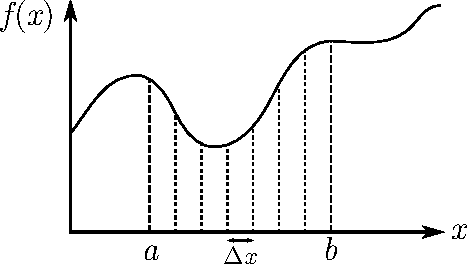
\includegraphics[width=0.4\textwidth]{./images/determinista}
	\caption{Discretització del domini de la funció en un mètode d'integració determinista}
	\label{fig:determinista}
\end{figure}

Per solucionar això, s'acostumen a fer servir mètodes d'integració aleatoris no depenen explícitament de cap discretització de l'espai.

%-----------------------------------------------------------------
\subsection{Mètodes aleatoris}
\subsubsection*{Mètode de l'encert--fallada}
Es tracta de generar punts $(\tilde{x},\tilde{y})$ seguint una distribució uniforme i comprovar si són per baix de la corba de la funció, és a dir, si es compleix $\tilde{y} < f(\tilde{x})$ (que compta com a un encert). Així doncs,
\begin{align}
	I = \int_{a}^{b} f(x) \dd{x} \Rightarrow \frac{I}{y_{0}(b-a)} \approx \frac{\text{nre. encerts}}{\text{nre. punts}}
\end{align}

\begin{figure}[H]
	\centering
	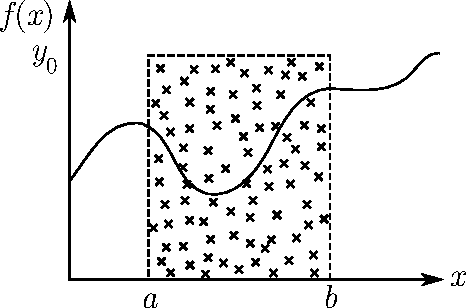
\includegraphics[width=0.4\textwidth]{./images/encert-fallada}
	\caption{Mètode d'encert--fallada}
	\label{fig:encert-fallada}
\end{figure}

\subsubsection*{Mètode de mostreig uniforme}
\begin{align}
	I = \int_{a}^{b} f(x) \dd{x} = I = \int_{a}^{b} \frac{F(x)}{b-a} \dd{x} = \ev{F}
\end{align}
on $F(x) = f(x) (b-a)$ és una funció coneguda.

Es tracta, doncs, de generar uniformement $x \in (a,b)$ i avaluar $F(x)$. Aquest mètode permet, fins i tot, avaluar la precisió del càlcul:
\begin{align*}
	I = \ev{F} \pm \frac{\sigma_{F}}{\sqrt{N}}
\end{align*}
on $\sigma_{F}$ és la desviació estàndard de cada punt mostrejat, i $N$ és el nombre total de punts mostrejats.

\subsubsection*{Mètode de mostreig general}
\begin{align}
	I = \int_{a}^{b} f(x) \dd{x} = I = \int_{a}^{b} F(x) g(x) \dd{x} = \ev{F}
\end{align}
on $g(x)$ és funció de distribució de probabilitat qualsevol ($g(x) \geq 0$, $\int_{a}^{b} g(x) \dd{x} \equiv 1$). Això permet mostrejar seguint la distribució que descriu $g(x)$ en comptes de fer-ho uniformement.

\begin{example}
	Si la funció $f(x)$ segueix alguna mena de distribució normal, interessaria donar més rellevància a uns punts que a uns altres. Això es podria fer fent un mostreig seguint una distribució $g(x)$ gaussiana, que es podria fer amb el mètode de Box--Muller.
	\begin{figure}[H]
		\centering
		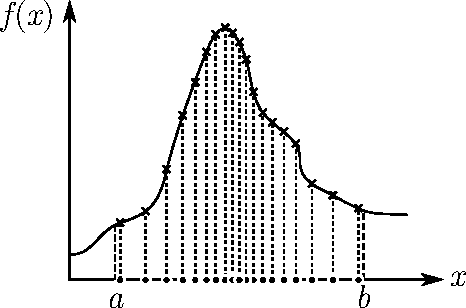
\includegraphics[width=0.4\textwidth]{./images/mostreig-gaussia}
		\caption{Mètode de mostreig seguint una funció de distribució de probabilitat $g(x)$ gaussiana}
		\label{fig:mostreig-gaussia}
	\end{figure}
\end{example}

%-----------------------------------------------------------------
\subsection{Generació de distribucions de probabilitat}
% \subsubsection*{Generació de distribucions de probabilitat}
Amb el mètode d'inversió, si disposem d'un generador de nombres aleatoris amb distribució uniforme $(0,1)$, podem obtenir variables aleatòries de qualsevol distribució de probabilitats.

\begin{thm}\label{thm:inversio}
	Donada una variable aleatòria $X$ amb una funció de distribució acumulada $G(x) = \int_{a}^{x} g(x) \dd{x}$, la variable $G(X)$ està, per definició, uniformement distribuïda en $(0,1)$. Aleshores, la variable aleatòria $G^{-1}(U)$ té funció de probabilitat acumulada $G(x)$ si $U$ està uniformement distribuïda en l'interval $(0,1)$.
\end{thm}

\begin{meth}[d'inversió]\label{meth:inversio}
	El teorema \ref{thm:inversio} ens diu que si podem invertir l'equació $u = G(x)$ per obtenir
	\begin{align}
		x = x(u) = G^{-1}(u)
	\end{align}
	podem generar nombres $x$ distribuïts com $g(x)$ si tenim nombres $u$ distribuïts uniformement en l'interval $(0,1)$.
\end{meth}

Un dels inconvenients que presenta aquest mètode és que no sempre es coneix la funció de distribució acumulada, o que no sempre és possible trobar una expressió adequada per a la inversa. A més a més, segons quina sigui l'expressió de la inversa, pot resultar lenta de calcular.

\begin{example}
	Considerem $X$ una variable aleatòria amb distribució exponencial de paràmetre $\lambda$, és a dir, amb funció de distribució de probabilitat
	\begin{align*}
		g(x) = \lambda e^{-\lambda x} \Rightarrow G(x) = 1 - e^{-\lambda x}
	\end{align*}
	Invertint aquesta funció, obtenim
	\begin{align*}
		Z \equiv - \frac{1}{\lambda} \ln(1 - U)
	\end{align*}
	Llavors, si $U$ està distribuïda de forma uniforme, la variable aleatòria $Z$ ho estarà de forma exponencial (figura \ref{fig:inversio-exp}).
	\begin{figure}[H]
		\centering
		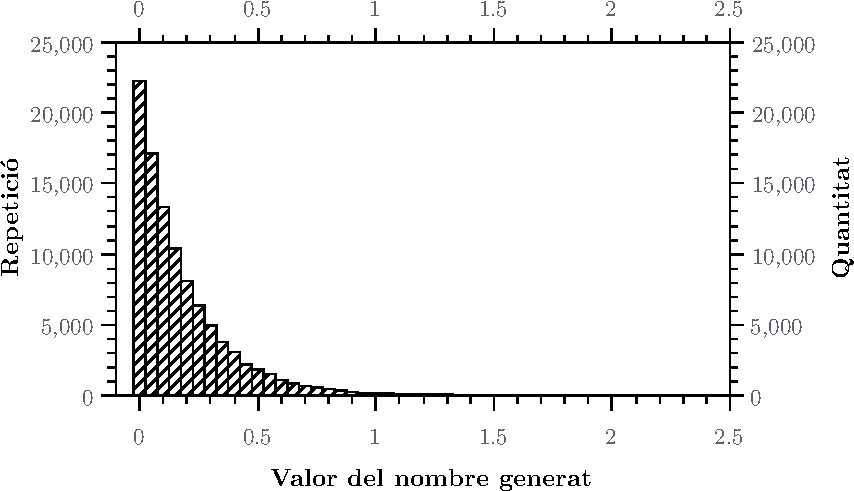
\includegraphics[width=0.74\textwidth]{./images/inversio-exp}
		\caption{Histograma dels \num{100000} nombres generats seguint una distribució exponencial amb $\lambda = 5$, emprant el mètode d'inversió}
		\label{fig:inversio-exp}
	\end{figure}
\end{example}

Es pot demostrar que emprar la funció de distribució $g(x) \sim f(x)$ per generar el mostreig minimitza l'error en el mètode d'integració (mostreig d'importància\footnote{En estadística, el mostreig d'importància és una tècnica general per a l'estimació de les propietats d'una distribució particular, tenint únicament mostres generades a partir d'una distribució diferent de la distribució d'interès.}). El problema és que idealment, $g(x) \equiv f(x) / \int_{a}^{b} f(x) \dd{x}$, que implicaria saber a priori el valor numèric de la integral, que és el que ens interessa trobar.

Una possible solució a aquest problema seria aproximar $g(x)$ a una funció més senzilla que la pròpia funció $f(x)$ (que comportaria possiblement un cert error), o bé, utilitzar mètodes de mostreigs dinàmics.

%-----------------------------------------------------------------
\subsection{Mètodes de mostreig dinàmics}
Ara el conjunt de punts a mostrejar $\qty{x_{1}, x_{2}, \dots, x_{n}}$ no està predeterminat, sinó que $x_{i+1}$ s'escull en funció del resultat de $x_{i}$.

Per implementar això s'utilitzen el que anomenem regles de rebuig o regles d'acceptació. La idea general de les regles de rebuig/acceptació és rebutjar/acceptar els punts $x_{i+1}$ depenent de si $f(x_{i+1})$ incrementa o disminueix respecte $f(x_{i})$, amb una certa probabilitat associada a l'acceptació.

\subsubsection*{Regles d'acceptació}
En comptes d'imposar $g(x) \sim f(x)$ ens podem conformar amb imposar que, si $\rho_{i}(x)$ és la distribució de probabilitat de $x_{i}$, llavors s'ha de complir
\begin{align*}
	\lim_{n \to \infty} \rho_{n}(x) \propto f(x)
\end{align*}

\begin{thm}[Condició de tallat de balanç]
	Una condició suficient per tenir la condició anterior és que es compleixi
	\begin{align*}
		\rho(x)p(x \to y) = \rho(y)p(y \to x)
	\end{align*}
	on $\rho(w)$ és la distribució de probabilitat de l'estat $w$, i $p(x \to y)$ és la probabilitat de transició $x \to y$.
\end{thm}

Segons les regles d'acceptació, tenim
\begin{align*}
	p(x \to y) = \alpha(x \to y) \acc{x}{y}
\end{align*}
on $\alpha$ és la probabilitat de mostrejar $y$ partint de $x$, i $\acc{x}{y}$ és la probabilitat d'acceptar aquest mostreig. Per simplicitat, s'acostuma a fer servir una regla de mostreig simètrica: $\alpha(x \to y) = \alpha(y \to x)$, de manera que s'ha de complir
\begin{align}
	\frac{\rho(x)}{\rho(y)} = \frac{\acc{y}{x}}{\acc{x}{y}}
\end{align}

\subsubsection*{Mètode de Metròpolis}
\begin{meth}[de Metròpolis clàssic]\label{meth:metropolis}
	Consisteix en agafar la regla d'acceptació seguint aquest criteri:
	\begin{align}
		\acc{x}{y} =
		\begin{cases}
			\rho(y)/\rho(x) & \rho(y) < \rho(x) \\
			1               & \rho(y) > \rho(x)
		\end{cases}
	\end{align}
\end{meth}

\begin{example}
	A la col·lectivitat canònica, tenim $\rho(\va{x}) = e^{- \beta H(\va{x})}/Z$. Llavors, es tracta de fer un canvi aleatori en una partícula (o conjunt de partícules), i acceptar el canvi seguint la següent regla d'acceptació:
	\begin{align*}
		\acc{\va{x}}{\va{y}} =
		\begin{cases}
			e^{- \beta \qty[H(\va{y}) - H(\va{x})]} & H(\va{y}) > H(\va{x}) \\
			1                                       & H(\va{y}) < H(\va{x})
		\end{cases}
	\end{align*}
	Observem que això té la mateixa interpretació física que esperaríem de la col·lectivitat canònica:
	\begin{itemize}
		\item Límit $T \to 0$ ($\beta \to \infty$): el sistema només accepta canvis que minimitzen l'energia:
		\begin{align*}
			\acc{\va{x}}{\va{y}} =
			\begin{cases}
				0 & H(\va{y}) > H(\va{x}) \\
				1 & H(\va{y}) < H(\va{x})
			\end{cases}
		\end{align*}
		\item Límit $T \to \infty$ ($\beta \to 0$): el sistema accepta tots els canvis, cosa que maximitza l'entropia.
	\end{itemize}
\end{example}

En simulacions de dinàmica molecular, segons les variables del sistema que es mantinguin constants, (de la mateixa manera que a la termodinàmica), podem definir diferents col·lectivitats.

\subsubsection*{Col·lectivitat $NVT$ (canònica)}
Apliquem un canvi aleatori en la posició\footnote{En general, només es canvia la posició, de manera que la velocitat de les partícules no pateix cap canvi aleatori.} d'una partícula (escollida aleatòriament), i utilitzem
\begin{align}
	\acc{\va{q}}{\va{q}\,\sast} =
	\begin{cases}
		e^{- \beta \qty[H(\va{q}, \va{p}) - H(\va{q}\,\sast, \va{p})]} & H(\va{q}\,\sast, \va{p}) > H(\va{q}, \va{p}) \\
		1 & H(\va{q}\,\sast, \va{p}) < H(\va{q}, \va{p})
	\end{cases}
\end{align}

\subsubsection*{Col·lectivitat $NPT$}
La col·lectivitat $NPT$ reprodueix les condicions experimentals típiques ($T$ i $P$ constants).
\begin{figure}[H]
	\centering
	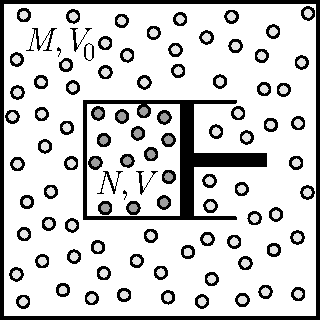
\includegraphics[width=0.25\textwidth]{./images/col-npt}
	\caption{Sistema amb dues regions amb pressió $P$ i temperatura $T$ constants}
	\label{fig:col-npt}
\end{figure}

Sabem que la funció de partició del sistema de la figura \ref{fig:col-npt}, suposant que les úniques variables d'interès són les de posició, és el producte de les funcions de partició de cadascuna de les dues regions:
\begin{flalign*}
	Z (N,V,T) &= Z_{1} \cdot Z_{2} = \frac{1}{h^{3N} N!} \int \dd{\va{q}} e^{-\beta H(\va{q})} \frac{1}{h^{3(M-N)} (M-N)!} \int \dd{\va{q}\,\sast} e^{-\beta H(\va{q}\,\sast)} &
\end{flalign*}
on $\va{q} = q_{1}, \dots, q_{N}$ i $\va{q}\,\sast = q_{N+1}, \dots, q_{M}$. Fent el canvi de variables $s_{i} = q_{i} / L$, i suposant que a la regió les partícules no interaccionen entre elles, obtenim
\begin{flalign*}
	Z &= \frac{V^{N}}{h^{3N} N!} \int \dd{s_{1}} \cdots \dd{s_{N}} e^{- \beta H(s_{1}, \dots, s_{N})} \frac{(V-V_{0})^{M-N}}{h^{3(M-N)} (M-N)!}. &
\end{flalign*}

Calculem ara el límit de $(V_{0} - V)^{M-N}$ considerant que $M \gg N$ i $V_ {0} \gg V$:
\begin{flalign*}
	\lim\qty{(V - V_{0})^{M-N}} &= \lim\qty{V_{0}^{M-N} \qty(1 - \frac{V}{V_{0}})^{M-N}} = V_{0}^{M-N} e^{-(M-N) V/V_{0}} & \\
	&\approx V_{0}^{M-N} e^{-\beta \rho V} = V_{0}^{M-N} e^{-\beta PV}.
\end{flalign*}

Així doncs, considerant que el volum $V$ és també una variable del sistema, la funció de partició es pot escriure com
\begin{flalign*}
	Z(N,P,T) &\propto \int \dd{V} \int \dd{s_{1}} \cdots \dd{s_{N}} e^{- \beta H(s_{1}, s_{N})} V^{N} e^{- \beta P V} = \int \dd{V} \int \dd{s_{1}} \cdots \dd{s_{N}} e^{- \beta H_{\text{eff}}} &
\end{flalign*}
on $H_{\text{eff}}$ és l'Hamiltonià efectiu:
\begin{align}
	H_{\text{eff}} = H + PV - \frac{N}{\beta} \ln V
\end{align}

Llavors ara podem emprar el mètode de Metròpolis amb l'Hamiltonià efectiu, $H_{\text{eff}}$:
\begin{align}
	\acc{\va{x}}{\va{y}} =
	\begin{cases}
		e^{- \beta \qty[H_{\text{eff}}(\va{y}) - H_{\text{eff}}(\va{x})]} & H_{\text{eff}}(\va{y}) > H_{\text{eff}}(\va{x}) \\
		1 & H_{\text{eff}}(\va{y}) < H_{\text{eff}}(\va{x})
	\end{cases}
\end{align}

\subsubsection*{Col·lectivitat de Gibbs}
És una barreja de les col·lectivitats $NVT$, $NPT$, i $\mu PT$. És important perquè és la manera més senzilla d'estudiar coexistència de fases.
\begin{figure}[H]
	\centering
	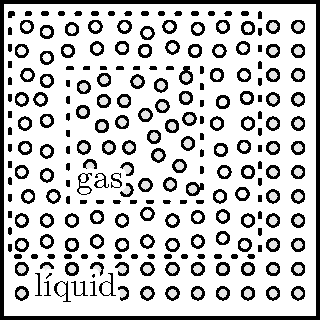
\includegraphics[width=0.26\textwidth]{./images/col-gibbs}
	\caption{Coexistància de fase gasosa i líquida}
	\label{fig:col-gibbs}
\end{figure}

Posant bé les condicions inicials, s'haurien de poder determinar bé cadascuna de les regions amb una fase determinada, però el problema és que la regió entre les fases és (i) inestable, i (ii) en general, molt ampla.

La col·lectivitat de Gibbs és l'única solució computacionalment ràpida per aquest problema (Panagiotopoulos, 1994). Al final, sense entrar en detalls en el desenvolupament, les regles d'acceptació de la col·lectivitat són:
\begin{subequations}
	\begin{itemize}
		\item Alteració aleatòria de la posició de la partícula:
		\begin{align}
			\acc{\va{x}}{\va{y}} =
			\begin{cases}
				e^{- \beta \qty[H(y) - H(x)]} & H(y) > H(x) \\
				1 & H(y) < H(x)
			\end{cases}
		\end{align}
		\item Alteració del volum:
		\begin{align}
			\acc{\va{x}}{\va{y}} =
			\begin{cases}
				\qty[\dfrac{V_{1}(y)}{V_{1}(x)}]^{N_{1} + 1} \qty[\dfrac{V_{2}(y)}{V_{2}(x)}]^{N_{2} + 1} e^{- \beta \qty[H(y) - H(x)]} & H(y) > H(x) \\
				1 & H(y) < H(x)
			\end{cases}
		\end{align}
		\item Alteració (intercanvi) de partícules:
		\begin{align}
			\acc{\va{x}}{\va{y}} =
			\begin{cases}
				\dfrac{N_{1}}{N_{2} + 1} \dfrac{V_{2}}{V_{1}} \, e^{- \beta \qty[H(y) - H(x)]} & H(y) > H(x) \\
				1 & H(y) < H(x)
			\end{cases}
		\end{align}
	\end{itemize}
\end{subequations}

